\chapter{Computational ASA}\label{chapter:casa}

Now, having described the underlying concepts from different fields of science in previous chapters, it is time to finally focus on computational auditory scene analysis. CASA is said to be the study that groups practical, programmable solutions for auditory scene analysis problems, or the study of ASA by computational means. CASA systems are used primarily for source se\-pa\-ra\-tion, meaning that they are machine listening systems that aim to separate "target" sounds from mixtures, just like people do when try to focus on a specific sound and not to be distracted by others. In that CASA systems differ from systems for blind signal separation – they try to mimic (at least to some extent) the mechanisms inside the human ear, which were discussed in chapter~\ref{chapter:biology}. In this chapter, main principles of CASA systems will be described, along with a typical architecture, goals and applications. In the second part, major works that use computational auditory scene analysis for source separation will be reviewed and compared.

\section{Principles, Goals and Applications}

Having the definition of CASA above, to be able to limit the requirements to the models it is necessary to describe the principles of CASA and common concepts across different systems. As the most major one, one could pick the restriction of number of microphones used in the input. Being based on the mechanisms of the human auditory system, CASA models only use recordings from one or two microphones (to simulate one or two ears), thus being split to monaural and binaural. Monaural models are researched better, but can't be used for extracting features based on the location of the sound, which is possible to some extent in binaural models, when time differences between the two recordings might be used.\\

To discuss the goals of CASA, it is useful to refer to the goals of ASA. According to Bregman~\cite{Bregman1990}, the primary goal of auditory scene analysis is to produce separate streams from the auditory input. Here, the term "stream" refers to a representation of a distinct sound source in the acoustic environment (see chapter \ref{section:biology_asa}), but, for example in \cite{Wang2006}, the authors also use it when talking about these representations in computer memory.\\

For CASA, Wang and colleagues \cite{Wang2005} proposed that the goal should be to find an ideal binary mask (IBM) for the time-frequency (T-F) representation of the input. If the input is split into T-F units, where time is on horizontal axis and frequency on vertical, the IBM is a binary matrix that has ones in places where the target sound is stronger, and zeroes elsewhere for background units. Ideal binary masks (and time-frequency masks overall) will be discussed in more detail in the following section.\\

The research of CASA systems and their applications in science \cite{Szabo2016} has been quite diverse recently. Some of the models are inspired by various biological experiments \cite{Wang2008}\cite{Boes2011}, while others are trying to address the cocktail party problem in natural environments \cite{Elhilali2008}. Some models try to explicitly simulate perceptual data, but others may refer to perception only very slightly. The expected output for the system implemented in this thesis is to find an IBM to be able to mask noisy background in monophonic piano music.\\

Aside from pure scientific interest, CASA systems find useful applications in everyday life \cite{Wang2006}. Some of them are listed below.

\begin{description}
	\item[Speech recognition] Apparently, speech recognition is the most popular field, where CASA systems have been used. Many speech recognition systems have performance losses in acoustic environments, where multiple sources of sound are present. The development is often put in contrast with computer vision systems that basically fulfill the same purpose, but for another human sense.
	\item[Automatic music transcription] A complex problem on its own (even human experts can come up with different solutions) becomes more complicated when multiple musical instruments are involved and need to be transcribed separately. CASA can certainly bring new insights to the field.
	\item[Hearing prostheses] Modern hearing aids made for people suffering from hearing loss don't separate speech in noisy environments, amplifying the noisy background too. CASA could address this problem to filter the noise out at least to some extent.
	\item[Audio information retrieval] Recordings on the Internet usually contain mixtures of sounds from different sources, thus it is necessary to separate them to be able to search efficiently.
\end{description}

\section{Typical Architecture}

The architecture described in the next subsections is based on \cite{Wang2006},  \cite{Wang2012} and \cite{Jasti2020}, though it is impossible to say that it is used in all systems -- in different sources the authors use different approaches and methods, and thus different structures of the models.

\subsection{Peripheral Analysis}

Usually, a model for computational auditory scene analysis begins with the peripheral analysis of the input sound. Here, the first preparations of the input sound for further processing take place. The expected result of this stage includes a time-frequency representation of the input sound -- a set of so-called T-F units. Since the models try to mimic the human cochlea --- and a lot of scientific attention was given to researching it --- the outcome of this stage is almost always a cochleagram.\\

Cochleagrams are in many cases produced by a filterbank of gammatone filters (see chap\-ter~\ref{section:math_concepts} for a definition). Gammatone filters were picked as the most precise ones to simulate points on the basilar membrane of the inner ear. The number of filters in the filterbank might be chosen by the researcher, but the most frequent choice is $128$. The center frequencies of the filters are distributed on the ERB-rate scale (see chapter \ref{section:math_concepts} for a definition), as it was developed to be similar with the critical-band scale of the human auditory system. The filters' impulse and frequency responses are shown on figure \ref{img:gammatone_filterbank}, however it is worth noting that the filters on the figure are normalized, and in practice frequencies higher than 2\,kHz are often amplified \cite{Wang2006}.

\begin{figure}[h]
	\centering
	\begin{subfigure}{0.48\textwidth}
		\centering
		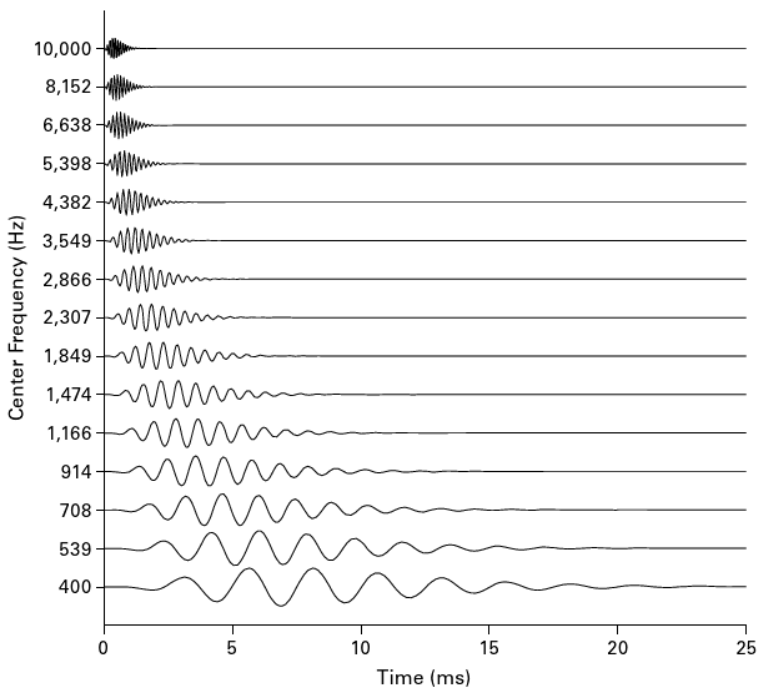
\includegraphics[width=\linewidth]{include/gammatone_filterbank_impulse_response}
		\caption{}
		\label{img:gammatone_filterbank_IR}
	\end{subfigure}%
	\begin{subfigure}{0.52\textwidth}
		\centering
		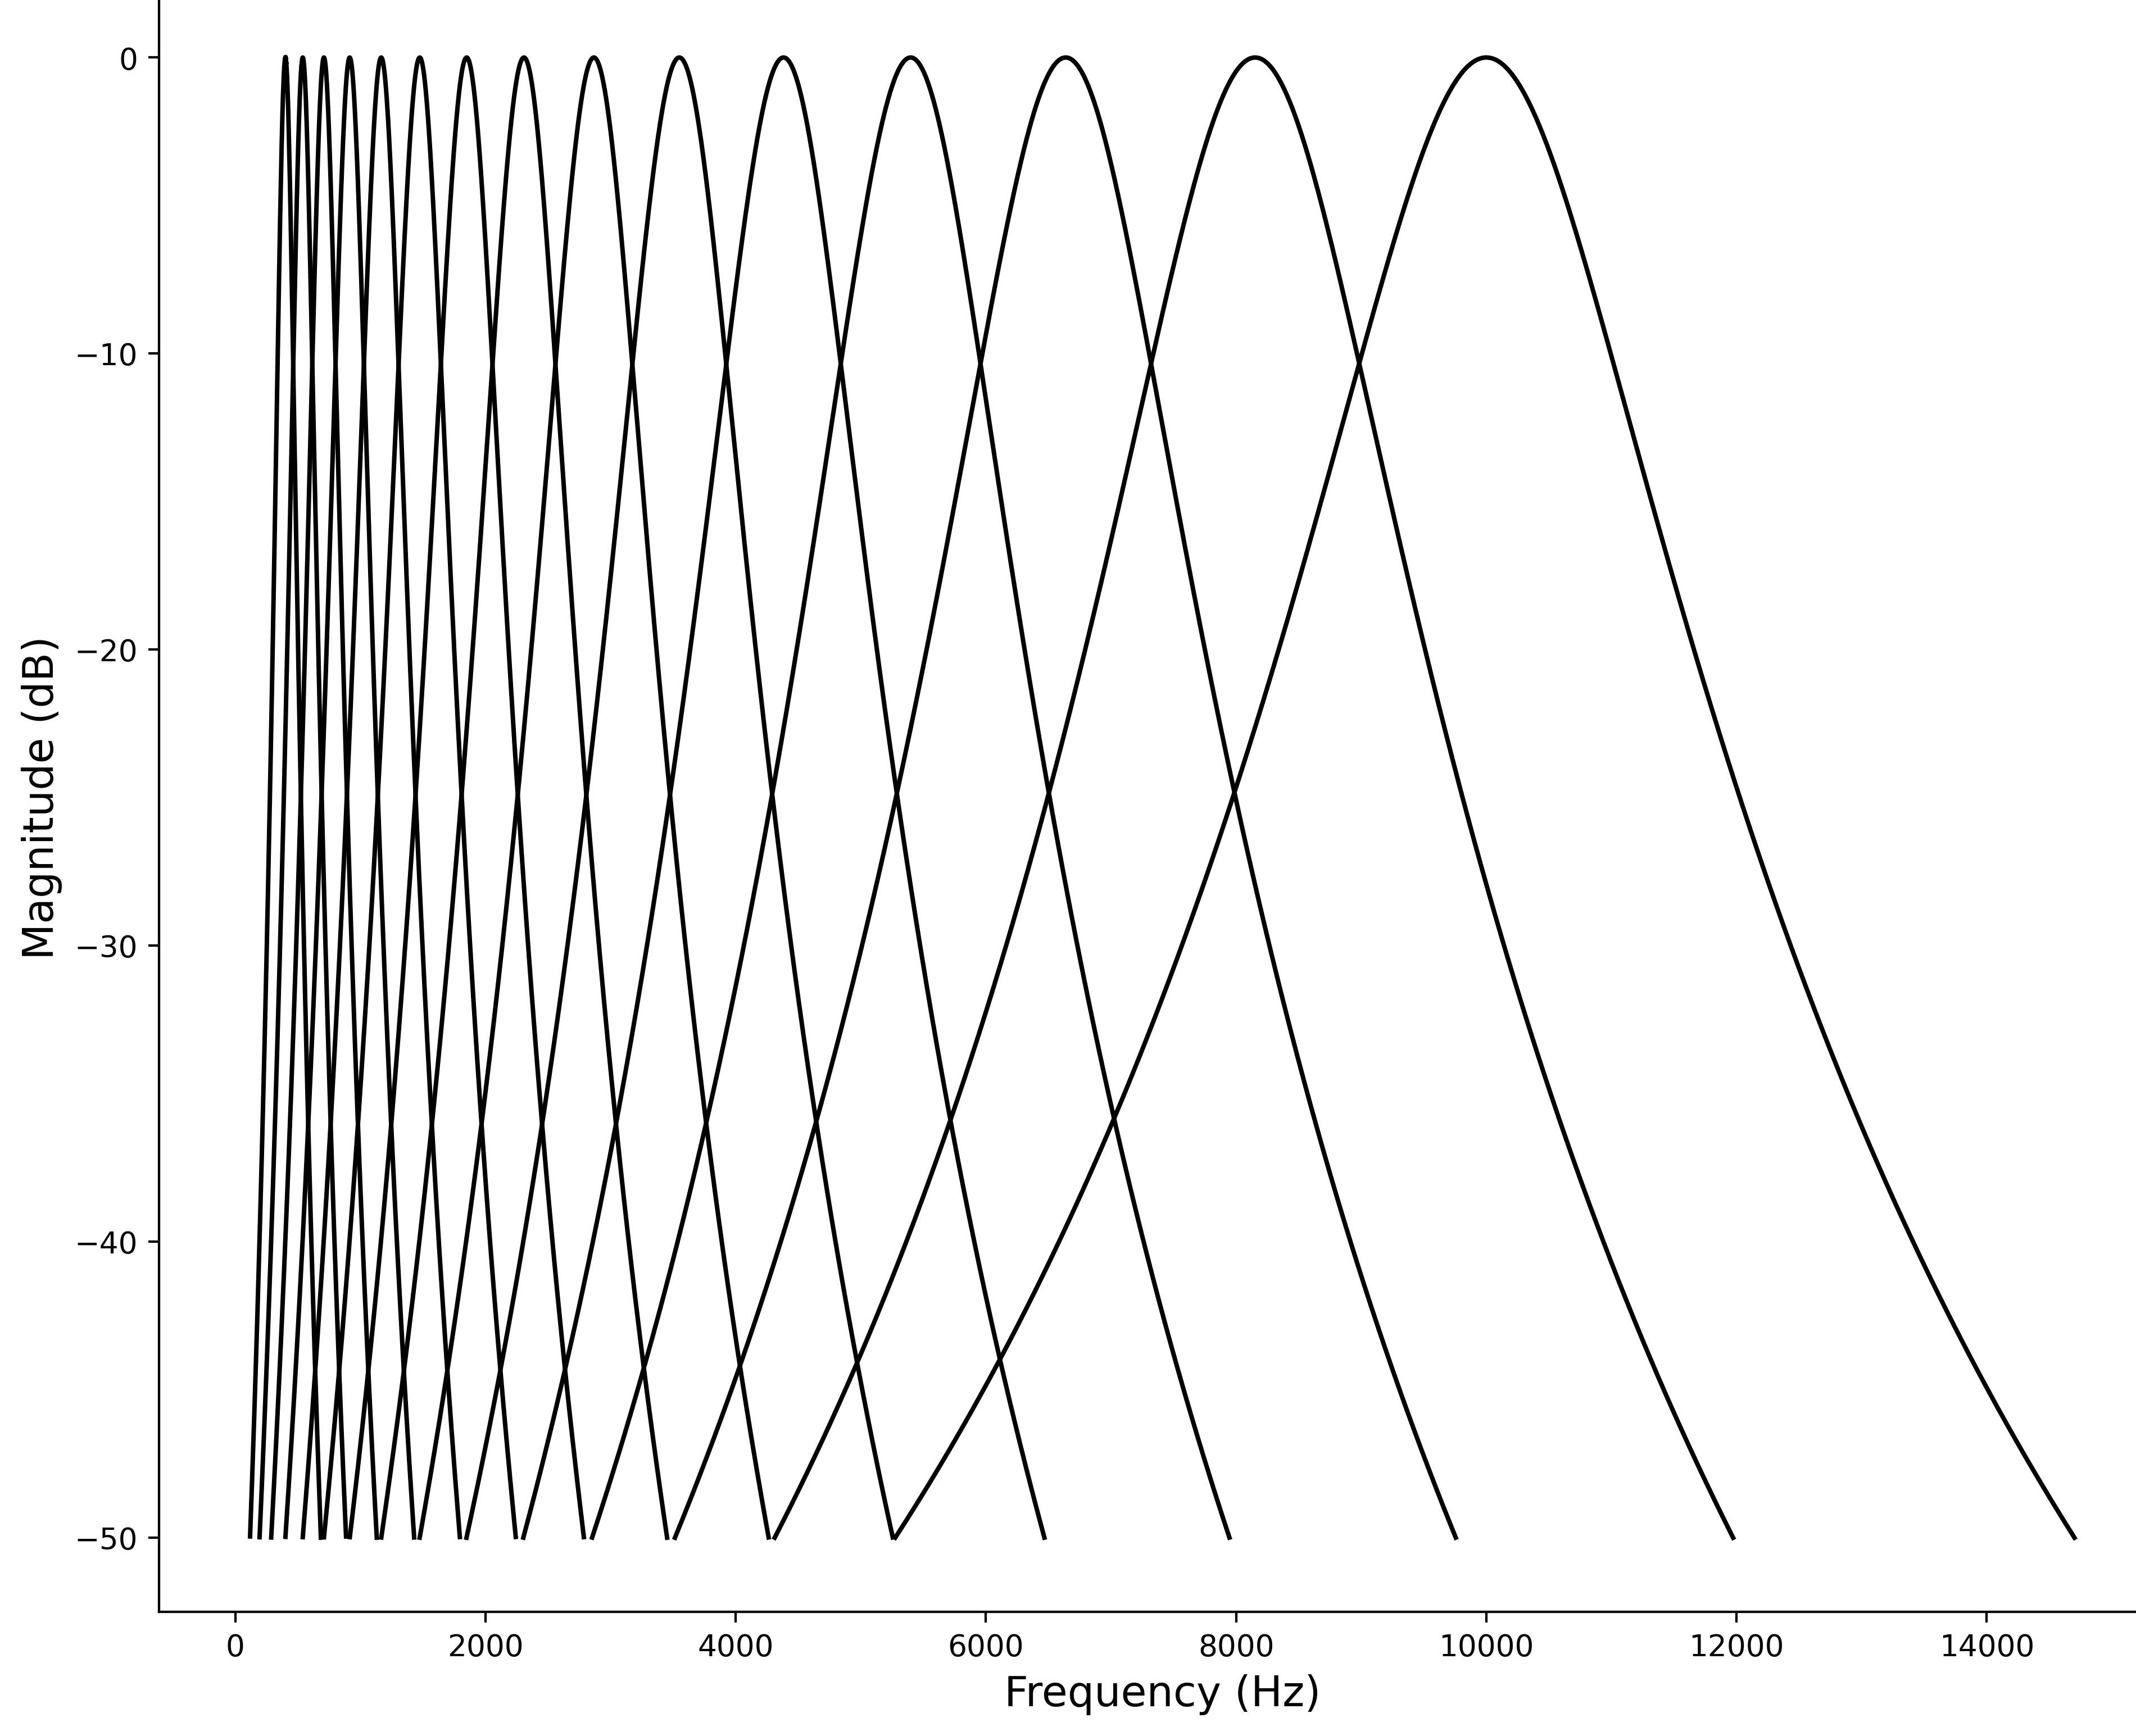
\includegraphics[width=\linewidth]{include/gammatone_filterbank_frequency_response}
		\caption{}
		\label{img:gammatone_filterbank_FR}
	\end{subfigure}
	\caption[Gammatone filterbank impulse and frequency responses]{\textbf{(a)} Impulse responses of $15$ gammatone filters in a gammatone filterbank. The filters' center frequencies are equally spaced between 400\,Hz and 10\,kHz on the ERB-rate scale and are shown on the vertical axis. Taken from \cite{Schnupp2011}. \textbf{(b)} Frequency responses of the same filters. The vertical axis depicts the changes in amplitudes in decibels. Note that the filters with higher center frequencies have wider bandwidths.}
	\label{img:gammatone_filterbank}
\end{figure}

If you look at a cochleagram and a spectrogram of the same sound at the same time, you probably won't notice many differences. The cochleagram similarly shows the densities of frequencies at different points in time, though in this case it may be thought of as a set of frequency channels, where each channel is the output of a certain gammatone filter from the filterbank. The gammatone filters are meant to change the signal so that the frequencies near the center frequency are kept, and the ones that are further away are attenuated (see figure \ref{img:gammatone_filterbank_FR}). At this stage, the windowing techniques described in chapter \ref{section:math_basics} are also used for long signals.

% TODO: Meddis hair cells?

\subsection{Feature Extraction}

After the cochleagram is computed, a classic CASA system involves computing a correlogram. In this thesis, correlograms will be put to the feature extraction stage, however some sources discuss them along with the cochleagrams in the peripheral analysis stage \cite{Jasti2020}.\\

According to \cite{Wang2006}, the term correlogram was introduced by Slaney and Lyon in 1990 \cite{Slaney1990} as \textit{"an animated picture of the sound that shows
frequency content along the vertical axis and time structure along
the horizontal axis"} (in this thesis the correlogram is a three-dimensional array). The authors used autocorrelation function (see chapter \ref{section:math_concepts} for a definition) on each frequency channel to compute it and described that if the sound is periodic, then the ACF will have peaks in places corresponding to the lags that are equal to the period of repetition. This property of the autocorrelation function has been extensively used in signal processing to estimate pitch and the corresponding fundamental frequencies.\\

So, the fundamental frequency is estimated using the correlogram and the representations of the higher harmonics in it. If you recall the conversation about harmonics from chapter \ref{section:physics_harmonics_pitch}, you may remember that harmonics are periodic at their fundamental frequency, so if the fundamental frequency is, for example, 100\,Hz (the period is 10\,ms), the second harmonic is 200\,Hz (5\,ms), and thus repeats every 10\,ms as well. The correlogram depicts this property in different frequency channels, and when the autocorrelations are summed up, the resulting summary ACF (see chapter \ref{section:math_concepts} for a definition) will have peaks in places corresponding to the period of the fundamental frequency.\\

Of course, correlogram might be used not only for the $f_0$-estimation. In the implementation part, for example, cross-channel correlation is computed from it too. Cross-channel correlation was defined in chapter \ref{section:math_concepts} according to \cite{Wang2012} and may be used to find similarities between units in adjacent frequency channels.\\

Some authors also work with cross-correlograms at this stage. According to \cite{Wang2006}, cross-correlogram is based on the simulated auditory nerve responses from the left and right ears (thus it may be used in binaural systems) and is defined as follows:
\begin{equation}
	CCF(n, c, \tau) = \sum_{k=0}^{K-1} a_L(n-k, c) a_R(n-k-\tau, c) h(k)
\end{equation}
where $a_L(n, c)$ and $a_R(n, c)$ is the above-mentioned simulated auditory nerve response from the left and right ears respectively, $\tau$ is the lag, $h(k)$ is the window function, and $K$ is the size of the sampling window.

\subsection{Mid-Level Representation and Scene Organization}

Next, after the feature extraction stage, follows some work related to segmentation and grouping, which according to Bregman are the main two stages of auditory scene analysis (see chapter \ref{section:biology_asa}). For this part, different authors come up with different names and implementations, but in this thesis it will be split into two stages as in \cite{Wang2006} and \cite{Jasti2020}: mid-level representation and scene organization.\\

Mid-level representation stage includes the first stage of Bregman's ASA --- segmentation. Here, the T-F units computed during the peripheral analysis stage are segregated into segments with the help of the extracted features. These segments, or mid-level representations, are meant to split the cochleagram into separate continuous parts and then are grouped to form auditory streams.\\

Scene organization stage, as it was mentioned, serves to group the mid-level representations into meaningful auditory objects, or streams (see chapter \ref{section:biology_asa}) that come from individual sound sources. Here, for example, separate harmonics are grouped together to form the richer musical sound, or the melody played by the pianist's right hand is grouped with the accompaniment played by the left hand. As a part of this stage, various techniques from the field of artificial intelligence might be used to achieve better results.\\

A notable outcome of this stage is a time-frequency mask of the input cochleagram (or any other chosen T-F representation). The main idea behind masking is to emphasize the T-F units corresponding to the target sound and attenuate those from the background. The mask might have either binary or real values from the $[0, 1]$ interval. If the former method is chosen, the task of searching the T-F mask might be interpreted as a binary classification problem. In case of the latter representation, the values from the mask might be interpreted differently: for example, as the signal-to-noise ratios (SNR) that show the ratios or differences between the target sound energy and overall energy in the T-F unit, or as probabilities that the T-F unit belongs to the target sound \cite{Wang2006}.\\

As it was mentioned earlier, Wang and colleagues \cite{Wang2005} proposed ideal binary mask (IBM) to be the primary goal of CASA. The IBM is defined as follows \cite{Wang2006}\cite{Wang2012}:
\begin{equation}
	IBM(n, c) = 
		\begin{cases}
			1 & \quad\text{if } SNR(n, c) \ge LC \\
			0 & \quad\text{otherwise}
		\end{cases}
\end{equation}
where $SNR(n, c)$ is the signal-to-noise ratio, or the difference between the target sound energy and the interference energy in the T-F unit, and $LC$ is the local criterion chosen as a threshold for the SNR function (most commonly 0\,dB).

\subsection{Resynthesis}

Finally, some systems include the resynthesis stage to convert the masked T-F representation back to the sound waveform. This is useful for the evaluation of the resulting CASA system in cases when listening experiments are held, or signal-to-noise ratios need to be compared before and after the processing \cite{Wang2006}. The technique for the resynthesis was proposed by Weintraub in his PhD~thesis in 1985 \cite{Weintraub1985}: the outputs from each gammatone filter in the filterbank were reversed in time to remove the phase shifts, then passed backwards through each filter and reversed back in time again.

\section{Major Works}
